\chapter{SPLICE - Software Product Line Integrated Construction Environment}
\label{ch:splice}

\begin{quotation}[Eight Mindful Steps to Happiness]{Henepola Gunaratana}
You alone are the author of your future. At every moment, you have the opportunity to change --- to alter your thoughts, your speech, your actions.
\end{quotation}


\section{Introduction}
The development of software products is a highly complex endeavor, which includes numerous interdependent activities, various different roles and a wide range of artifacts spanning over all phases and activities \citep{lacheiner2011}.

In this chapter, we present functional and non-functional requirements for a tool, it architecture, involved frameworks and technologies, and its implementation. The tool is called \acf{SPLICE}, built in order to support and integrate \ac{SPL} activities, such as, requirements management, architecture, coding, testing, tracking, and release management, providing process automation and traceability across the process.

We also present a metamodel, which proposes a representation of the \ac{SPL} artifacts, based on agile methods  and variability management amount the assets (Features, Requirements, Use Case, etc...). This metamodel is implemented by \ac{SPLICE}.

The remainder of this chapter is organized as follows: \secref{sc:requiriments} presents the requirements of the tool; \secref{sc:metamodel} describes the created SPL metamodel; \secref{sc:architecture} shows its general architecture; details of the implementation are discussed in \secref{sc:implementation}; \secref{sc:inaction} shows the tool in operation; and, finally, \secref{sc:splicesummary} presents the summary of the chapter.



\section{Tool Requirements}
\label{sc:requiriments}
\subsection{Functional Requirements}

According to \cite{Sommerville2007} , Functional Requirements are statements of services the system should provide, how the system should react to particular inputs, and how the system should behave in particular situations. In the \ac{SPLICE} specification, the following functional requirements were defined:

\begin{itemize}
\item  \textbf{FR1 - Traceability of lifecycle artifacts.} The tool should identify and  maintain relationships between managed lifecycle artifacts. It is also important not just for reporting but also for enabling change impact analysis and information visibility through the development lifecycle.

\item  \textbf{FR2 - Reporting of lifecycle artifacts.} It must use lifecycle artifacts and traceability information to generate needed reports from the lifecycle product information. Thus, supporting the \ac{SW} development and management and easily producing ready to consume documentation for the stakeholders.



\item  \textbf{FR3 - Metamodel Implementation.} The \ac{SPLICE} should implement the entities and relationships described in a defined metamodel. The metamodel created comprises the relationships among the SPL assets, allows traceability and facilitate the evolution and maintenance of the SPL. This requirement is very demanding and complex, and include a big number of features to correctly represent the metamodel presented, such as \textit{Product Map}, \textit{Features Selection} and \textit{Evolution management}.


\item  \textbf{FR4 - Issue Tracking.} Issue Tracking play a central role in software development, and the tool must support it. It is used by developers to support collaborative bug fixing and the implementation of new features. In addition, it is also used by other stakeholders such as managers, QA experts, and end-users for tasks such as project management, communication and discussion, code reviews, and story tracking \citep{Baysal2013}.
 
\item  \textbf{FR5 - Agile Planning.} In the software industry, there is a strong shift from traditional phase-based development towards agile methods and practices. Some of agile characteristics includes: customer collaboration, small self-organizing teams, emphasis on coding, minimal bureaucracy and documentation effort, test-driven development, and incremental delivery \citep{Hochmuller2011}.

\item  \textbf{ FR6 - Configuration management.} For evolution management, the tool must support change management across all the managed artifacts. It must also support creating and controlling the mainstream version management systems such as CVS, SVN and GIT. 

\item  \textbf{ FR7 - Unified User management.}  As an integrated environment, with the plan to cover all the lifecycle activities, the tool can use a number of external tools, taking advantage of the vibrant community and quality present in some open-source/freely available tools. For convenience, it must provide a unified user management between all the tools.

\item  \textbf{ FR8 - Collaborative documentation.}  Wiki is a collaborative authoring system for collective intelligence which is quickly gaining popularity in content publication and it is a good candidate for documentation creation. Wikis collaborative features and markup language make it very appropriate for documentation of Software Development tasks. 

\item  \textbf{ FR9 - Artifacts search.} All artifacts managed by the tool must support keyword search, and present the results in an adequate way.
\end{itemize}

\subsection{ Non-Functional Requirements}

\cite{Sommerville2011} define Non-Functional Requirements as requirements that are not directly concerned with the specific services delivered by the system to its users. They place restrictions on the product and the development process, and specify constraints that the product must meet. Non-functional requirements of the tool is described as follows:

\begin{itemize}
\item  \textbf{ NFR1 - Web-based interface. } A web-based tool enables a high level of interoperability between different systems. It allows engineers and stakeholders to collaborate and access the system independently of their location.

\item  \textbf{ NFR2 - Metamodel Flexibility. } There is no perfect process, and metamodels changes and evolves quickly. The tool must be implemented in a way to easily allow metamodel changes.


\item  \textbf{ NFR3 - Extensibility. } The \ac{SPLICE} must have a plugin infrastructure for allowing external developers to interact with it using an API. It is planned that in the future, the \ac{SPLICE} could become a platform which enable undergraduate students to build and performs Software Engineer experiments on it.

\item  \textbf{ NFR4 - Usability. } As an integrated environment, it will aggregate a plethora of different tools. It is important to have a consistent User Experience between them. The tool must also conform with the latest trends in web-design, and must provide a modern and minimalist interface.

\item  \textbf{ NFR5 - Accountability. } All users actions must be logged, for evolution management, security and accountability. 

\item  \textbf{ NFR6 - Transparency. } The user must identify the collection of tools as a single tool. The tool must permit that all the integrated tools be accessible with just one login.

\item  \textbf{ NFR7 - Security. } Being web-based and publicly accessible, it is necessary to keep a tight access control in the application in order to guarantee the privacy and confidentiality of the projects.


\end{itemize}


\section{A lightweight SPL metamodel}
\label{sc:metamodel}
\begin{figure}[htp]
\begin{center}
  \includegraphics[width=16cm]{chapters/proposed_solution/img/diagram.png}
  \caption[\ac{SPLICE} Metamodel]{\ac{SPLICE} metamodel}
  \label{fg:metamodel}
\end{center}
\end{figure}



A \acf{SPL} process has to handle interconnected and complex models such as feature and architecture models. Furthermore, traceability is fundamental to ensure that they are consistent. An efficient process require mature software engineering, planning and reuse, adequate practices of management and development, and also the ability to deal with organizational issues and architectural complexity. \citep{Birk2007}.

To address the previously defined function and non-functional requirements, we decided to use a model-driven approach to represent all the information, activities and connections among artifacts. With a well-defined metamodel we can provide automation and interactive tool support to aid the corresponding activities.

A huge number of metamodels have been proposed in the literature in the past \citep{Schubanz2013, Araujo2013, Anquetil2010, Bayer2001, Buhne2005, Seidl2012}, including one done by a \ac{RiSE} researcher \citep{Cavalcanti:2011}. However, we found that all the metamodels propose a heavyweight and formal process, and do not fit with a more lightweight and informal methodology such as agile methods.

\begin{figure}[htp]
\centering
\includegraphics[width=23cm, angle=90]{chapters/proposed_solution/img/full_diagram.png}
  \caption[Django generated UML]{Django generated meta-model}
\label{fg:output}
\end{figure}
In the \figref{fg:metamodel} we propose a lightweight metamodel, adapted from \citet{Cavalcanti:2011}, representing the interactions among the assets of a SPL, developed in order to provide a way of managing traceability and variability, however it explicitly removes, for clarity, the representation of user-management, authentication, Version control, Issue Tracking,  Logging and internal models.A more complete diagram is depicted on \figref{fg:output}. The proposed metamodel represent diverse reusable assets involved in a SPL project, and there are five sub-models:

\begin{itemize}
\item  \textbf{ Scoping Module } In this module, is located the core of the metamodel, the Feature and the Product Model. Many artifacts relates directly with the Feature Model including \textit{Use Case},  \textit{Glossary}, \textit{User Story} and \textit{Scope Backlog}. A  \textit{Product} is composed of one or more \textit{Features}.

The \textit{feature} model is represented as a Modified Preorder Tree Traversal, which allow representing hierarchies. This is used to model relationships between features. It also permit \textit{required} and \textit{excluded} features relationships. \textit{Feature} also have a \textit{Glossary}, containing the definition of terms used. Additionally it have \textit{BindingTime} and \textit{VariabilityType} values associated with it. \cite{Kang1990} describes examples of \textit{binding time}, such as \textit{before compilation}, \textit{compile time}, \textit{link time}, \textit{load time}, \textit{run-time}; and examples of variability as \textit{Mandatory}, \textit{Alternative}, \textit{Optional}, and \textit{Or}.

The Scoping module also have a \textit{ScopeBacklog} model, that permit to classify the features by order of importance. 

\item  \textbf{ Requirements Module }
The metamodel also involves the requirement engineering traceability and interactions issues, considering the variability and commonality in the SPL products \citep{CavalcantiInTech2012}. The main object of this SPL phase is \textit{Use Case}. Differently from \cite{CavalcantiInTech2012} metamodel, we following an agile development process, which has been designed to cope with requirements that changes during the development process. In these processes, when a user proposes a requirements change, this change does not go through a formal change management process.

The \textit{Use Case} model is composed by \textit{description}, \textit{precondition},  \textit{title} and a number of  \textit{MainSteps} and  \textit{AlternativeSteps}
The concept of \textit{ User stories } is used in this metamodel to represent what a user does or needs to do as part of his or her job function. It is composed by a \textit{name} and the associated template : \textit{As a},   \textit{I want} and \textit{So that}.

\item  \textbf{ Testing Module }
An agile project is centered on short iterations in which each iteration can be viewed as a small project of its own. Therefore, one characteristic of an agile project is the high degree of rework that mandates a comprehensive set of regression tests \citep{Goeschl2010}.

According to \cite{Shaye2008}, test automation plays the greatest role in agile testing, with it is possible to keep testing and development in synchronization.
In the metamodel proposed we represent the usual test workflow in agile environments. The \textit{Test Case} model is related to one \textit{Use Case} and is composed of a \textit{name}, \textit{description}, the \textit{Expected result} and a set of \textit{Test Steps}. One \textit{Test Case} can have many \textit{Test Execution} that represent one execution of it.  The reasoning for the \textit{Test Execution} is to enable a test automation machinery.

The metamodel also represent the acceptance testing with the \textit{Acceptance Test} and \textit{ Acceptance Test Execution}.  An acceptance test is a formal description of the behavior of a software product, usually expressed as an example or a usage scenario. In principle, the customer or his representative is given the role of expressing requirements as input to the software paired with some expected result \citep{Shaye2008}.  The \textit{Acceptance Test} model is based on the \textit{Given-When-Then} template. (Given) some context, (When) some action is carried out, (Then) a particular set of observable consequences should obtain. It also have a number of \textit{Acceptance Test Execution} associated with it. The \textit{Acceptance Test Execution} is composed of the date it was executed, test result and the observations.
\item  \textbf{ Agile Planning Module }
There are several product development approaches, such as agile, interactive, incremental, and phased approaches. This metamodel is more closely related to an agile methodology, which is an incremental and iterative style of development, with focus on customer collaboration. In agile software development, the project is developed in a series of relatively small tasks, visualized, planned and executed by producing a shippable incremental product for the customer \citep{Uikey2012}.

The agile interactions are called \textit{sprints}, and there are an upfront planning of it, represented in the metamodel by the \textit{Sprint Planning} model. This planning is composed of a number of \textit{Tickets}, a \textit{deadline}, an \textit{objective} and a \textit{start date}. At the end of the sprint, it happens a retrospective, represented in the model by \textit{Sprint Retrospective}, that contains a set of \textit{Strong Points} and \textit{Should be Improved} models that express what points in the spring was adequate, and what needs improvement. 
\item  \textbf{ Others Module }
This module is composed of all the models that did not fit in the other sections. It includes \textit{Wiki} model for a collaborative document creation; \textit{Ticket} model for Issue tracking; and \textit{Milestone}, \textit{Version}, \textit{Note} for release management.

\end{itemize}





\section{SPLICE Architecture and Technologies}
\label{sc:architecture}

\begin{figure}[htp]
\begin{center}
  \includegraphics[width=15cm]{chapters/proposed_solution/img/architecture.png}
  \caption[SPLICE architecture overview]{SPLICE architecture overview }
  \label{fg:splice-architecture}
\end{center}
\end{figure}


\subsection{Architecture Overview}



The \ac{SPLICE} architecture was planned to cover all the essential steps of the \acf{SPL} process, coping with the defined functional and non-functional requirements and acting as a \acf{ALM} tool.  During the evaluation of existing tools in \secref{sc:relatedWork}, we found in that the tool \textit{Trac \footnote{http://trac.edgewall.org}} was a perfect candidate to be the base of our product. \textit{Trac} is an open source, Web-based project management and bug tracking system .It has been chosen for a number of reasons:
\begin{itemize}
\item  \textbf{Stable and Established tool.} \textit{Trac} initial release was on October 1, 2006, and the version 1.0, defined as stable, was released 7 years after. Its source has been deeply scrutinized for issues and a number of high-value users have public accessible instances of \textit{trac}. Trac is reported to have more than 450 major installations worldwide \footnote{http://trac.edgewall.org/wiki/TracUsers}.Some notable users includes NASA's Jet Propulsion Laboratory\footnote{http://www.jpl.nasa.gov/}  , Nginx\footnote{http://trac.nginx.org/nginx/} and WordPress \footnote{https://core.trac.wordpress.org/}. Thus, we have good indicators of stability and security.

\item  \textbf{Extensible with a thriving ecosystem.} \textit{Trac} is extensible via plugins. Plugins can be used to add functionality that was not previously possible without extensive modification to the source. The website Trac-Hacks \footnote{http://trac-hacks.org/wiki/HackIndex} indexes more than 600 plugins, that includes a wide range of functionality, such as: extended milestone facilities; multi-project functionality; integration of automated build systems; dependency graphs and Distributed Peer Review.
This makes very likely that for many popular requests, may already exist a plugin that provides the wanted functionality.

\item  \textbf{Set of features.} 
After examination if other open-source solutions, we found that \textit{Trac} had a good number of features needed to build our tool. \textit{Trac} defines\footnote{http://trac.edgewall.org/} itself as an "enhanced wiki and issue tracking system for software development projects". It provides: an interface to Subversion and Git (or other version control systems), an integrated Wiki and convenient reporting facilities. Trac also allows wiki markup in issue descriptions and commit messages, creating links and seamless references between bugs, tasks, changesets, files and wiki pages. Futhermore, \textit{trac} have a timeline showing all current and past project events in a temporal order, making the acquisition of an overview of the project and tracking progress very easy. 

\item  \textbf{ Liberal license. } \textit{Trac} uses the Revised BSD License \footnote{http://opensource.org/licenses/BSD-3-Clause} , a very permissive free software license, imposing minimal restrictions on the redistribution of covered software. This enable us to modify and distribute the code without any restriction.

\end{itemize}

An overview of the architecture of \ac{SPLICE} can be seen in \figref{fg:splice-architecture}. Using the \textit{Trac} tool as foundation to the \ac{SPLICE} tool, two separated modules were built to provide the missing functionality. \textit{Tonho}, is our main module, where all the metamodel and functionality not provided by \textit{Trac} is implemented and the \textit{Authentication manager} is the module who provides the \textit{Single sign-on} property among the tools, supplying unified access control with a single login.

All the bridge between \textit{Tonho} and \textit{Trac} is made using plugins, a shared database and templates. Absolutely no modification was done to \textit{Trac} core. This solution permits to easily upgrade \textit{Trac} in the future taking advantage of new features and security fixes.	All modules of the architecture share the same Database and have the same template design.  Each component of the architecture is detailed in the following section.


\subsection{Architecture Components}
The architecture of the tool is composed of the \textit{Trac}, a core (\textit{Tonho}) module, a database module, an Authentication Control (\textit{Maculelê}) module and a set of versioning and revision control tools.

 \figref{fg:splice-architecture} illustrates a simplified organization of the architecture of the application: the \textbf{\textit{Authentication Control}} validates the request and enable access to the tools if the user have the right credentials; \textbf{\textit{Trac}} is responsible for Issue Tracking, managing the versioning and revision control tools, collaborative documentation and plugin extensibility; the main module \textbf{(\textit{Tonho})},it is where the metamodel is implemented and has sub-modules for each metamodel module, such as: \acf{SC}, \acf{RQ}, \acf{TE}, \acf{AP} and \acf{OT};\textbf{ \textit {Versioning and revision control}} is part of  software configuration management, and is composed of the set of external \acf{VCS} tools such as \textit{SVN}, \textit{GIT} and \textit{Mercurial}. It tracks and provides control over changes to source code, documents and other collections of information; and finally, the \textbf{\textit{Database}} stores in an organized way all the asserts and do the persistence of the data among the tools. Next, it will be provided more details for each component.

\textbf{Trac}. \textit{Trac} is a minimalistic web-based software project management and bug/issue tracking system. It is the foundation and it development is completely external to the \ac{SPLICE} tool development. It was the initial module important to the architecture and provides an interface to the revision control systems, an integrated wiki, flexible issue tracking and convenient report facilities. 
The communication with the rest of the modules is done by the shared database, and a set of plugins developed to make a bridge between the rest of the architecture. Internally \textit{Trac} the following technologies to archive it goal:
\begin{itemize}

\item  \textbf{ Genshi.} Genshi is a Python library that provides an integrated set of components for parsing, generating, and processing HTML, XML or other textual content for output generation on the web. \footnote{http://genshi.edgewall.org/} It is used in \textit{Trac} to provide templating and representing any information to the user. 



\item  \textbf{ SWIG bindings .} Many popular \acf{VCS} are set of C libraries, for example Subversion and Git. As \textit{Trac} is developed using the Python scripting language, it cannot directly use those libraries. It need a tool to allow calling native functions. \acf{SWIG} is an open source software tool used to connect computer programs or libraries written in C or C++ with scripting languages such as Python and is used in \textit{Trac} to enable access to popular \ac{VCS} such as  \textit{SVN}, \textit{GIT} and \textit{Mercurial}.

\end{itemize}

\begin{figure}[htp]
\begin{center}
  \includegraphics[width=15cm]{chapters/proposed_solution/img/django-admin.png}
  \caption[SPLICE model transformation]{SPLICE model transformation}
  \label{fg:splice-django-admin}
\end{center}
\end{figure}


\begin{figure}[htp]
\begin{center}
  \includegraphics[width=10cm]{chapters/proposed_solution/img/django-class.png}
  \caption[SPLICE Model Class]{ SPLICE model class }
  \label{fg:splice-django-class}
\end{center}
\end{figure}


\textbf{\ac{SPLICE} Tonho.} \textit{Tonho} is the internal codename for the core module of \ac{SPLICE}, where all the functionality missing from \textit{Trac} and the proposed metamodel is implemented. The non-functional requirement NFR2, required Metamodel Flexibility, and this module was carefully designed to be flexible and easily allow future metamodel alterations.  

The idea is at the begin of each project, the Software Engineer would describe the metamodel he wanted for that specific project. He may choose to use a predefined metamodel, such as the one presented here, or to customize it adding, removing or modifying assets.

An overview of the solution can be seen in \figref{fg:splice-django-admin}. The \ac{SPLICE} will ship a public accessible set of classes that represent the metamodel, and the engineer can modify the metamodel, by changing the objects fields names, types and descriptions. 

A \acf{ORM} module will then convert the class model and create a database representing all the relations in a SQL format. Finally a tool will automatically read the metadata in the models and using the created database, will provide a powerful and production-ready "\acf{CRUD}" interface. \figref{fg:splice-django-class} exemplify how this a class look like. This gives unprecedented level of flexibility, as the metamodel can be changed without any other effort then direct modifying the models. The set of technologies used to possibility this were:


\begin{figure}[htp]
\begin{center}
  \includegraphics[width=6cm]{chapters/proposed_solution/img/django-architecture.png}
  \caption[Django Architecture]{Django Architecture}
  \label{fg:django-architecture}
\end{center}
\end{figure}


\begin{itemize}
\item  \textbf{ Django.} For creating the web-application, we choose the Django Framework. It is a high-level Python Web framework that encourages rapid development and pragmatic design that follows the Model-View-Controller (MVC) pattern.
Between a number of frameworks available for \textit{Python} web-development, Django was chosen because it employs and enforces a model-view-controller (MVC) methodology, a common development pattern for separating presentation from application logic,  encouraging good development practices and produces a more maintainable code. An overview of Django architecture can be seen in \figref{fg:django-architecture}. Django is also the most widely used Python web framework, with a very well established community of developers.

The \ac{SPLICE} also relies on Django \acf{ORM}, where the metamodel is mapped as entities and their relationship into Python classes and the \ac{ORM} automatically create a relational database.

\item  \textbf{ Bootstrap.} The interface and design were build using the Bootstrap Framework\footnote{http://getbootstrap.com}. Bootstrap is a free collection of tools for creating websites and web applications. It contains HTML and CSS-based design templates for typography, forms, buttons, navigation and other interface components, as well as optional JavaScript extensions\footnote{http://en.wikipedia.org/wiki/Bootstrap}.
\end{itemize}


\textbf{\ac{SPLICE} Database}
The database is a central point of the whole architecture. It is shared between two major modules, and permit global access to assets and informations. This characteristic is very important to provide traceability and enable creation of detailed and complete reports among a variety of assets, produced by different modules. The technology used to implement the database was:
\begin{itemize}
\item  \textbf{ SQLite.} To implement the database of the application, it was chosen the SQLite database. It is a powerful, embedded relational database management system in a compact C library. It offers support for a large subset of SQL92, multiple tables and indexes, transactions, views, triggers and a vast array of client interfaces and drivers. The library is self-contained, fast, efficient and scalable. 

\end{itemize}

\textbf{\ac{SPLICE} Authentication Control (\textit{Maculelê}) }
This module is responsible for coordinating the authentication and control access between the modules, satisfying the requirement \textit{usability}. It have a Single sign-on property and the \ac{SPLICE} tool provides a control panel that manages all users accounts. 

The user-session is stored as a cookie sent to the user browser, it is composed of the user-metadata and a US Secure Hash Algorithm 1 (SHA1) hash of the user meta-data with a secret code stored on the server, protecting from forgery while giving persistence of credentials. 

\textbf{Versioning and revision control }
Version management is an important part of the Configuration management process. It is the process of keeping track of different versions of software components or configuration items and the systems in which these components are used. It also involves ensuring that changes made by different developers to these assets do not interfere with each other. To support version management, you should always use \acf{VCS} tools \citep{Sommerville2011}. \ac{VCS} are external modules from the architecture with the communication bridged by \textit{SWIG} bindings.  \ac{SPLICE} provides support for two popular \ac{VCS} systems: \textit{SVN} and \textit{GIT}. 





\section{Implementation}
\label{sc:implementation}


The proposed tool was implemented using the Django Framework and the Python programming language. According to \cite{python2014}, “Python is a dynamic object-oriented programming language that is used in a wide variety of application domains. It have  a very clear, readable syntax,  offers strong support for integration with other languages and tools, comes with extensive standard libraries, and can be learned in a few days. Many Python programmers report substantial productivity gains and feel the language encourages the development of higher quality, more maintainable code”.

The motivation for choosing this stack was because the \textit{trac} was already build with Python and the unprecedented flexibility that the Django \acf{ORM} empowers it users, making the metamodel changes effortless. Python is also becoming the introductory language for a number of computer science curriculums \citep{Sanders2008}. Python is also frequently used on many scientific workflows \citep{Bui2010} making the project attractive for future data scientists experiments and for undergraduate projects. Other languages used to developed the tool were JavaScript, CSS, HTML, XML, YAML and make.

\begin{table}
\begin{center}
    \begin{tabular}{|l|l|l|l|l|}
    \hline
    Language   & Files & Blank lines & Comment lines & Code lines  \\ \hline
    Javascript & 105   & 6746  & 5064    & 27421 \\ 
    CSS        & 59    & 3021  & 646     & 20588 \\ 
    Python     & 147   & 3115  & 3400    & 13903 \\ 
    HTML       & 134   & 836   & 148     & 7154  \\ 
    XML        & 10    & 8     & 0       & 797   \\ 
    YAML       & 1    & 0     & 0       & 11   \\ 
    make       & 1     & 3     & 1       & 9     \\ \hline
    Total      & 457   & 13729 & 9259    & 69883 \\ \hline
    \end{tabular}
    \caption{Project statistics}
    \label{table:statistics}
    \end{center}
\end{table}


The \ac{SPLICE} tool was developed by only one person and it took about 8 months of intensive development (30 hours/week). According to cloc tool \footnote{http://cloc.sourceforge.net} , the \ac{SPLICE} project consists of almost 70k lines of code, excluding comments and blank lines. Table \ref{table:statistics} shows the code statistics of the project. All the \ac{SPLICE} code is platform-independent, and has been thoroughly tested on both Windows and Linux environments. 






\section{SPLICE in action}
\label{sc:inaction}

\begin{figure}[htp]
\begin{center}
  \includegraphics[width=16cm]{chapters/proposed_solution/img/splice-features.png}
  \caption[SPLICE features]{SPLICE features}
  \label{fg:splice-features}
\end{center}
\end{figure}

The \ac{SPLICE} is a complex tool, covering many steps and different process, and work as a façade for a number of external tools. In order to demonstrate how the tool works, this section shows the operation of a number of selected features, with a brief description. \figref{fg:splice-features} depicts some features offered by the \ac{SPLICE} and what came from \textit{trac}. The tool, following the non-functional requirement \textit{NFR1 - Web-based interface}, is a web-based tool.

\subsubsection{Main Screen}
\begin{figure}[htp]
\begin{center}
  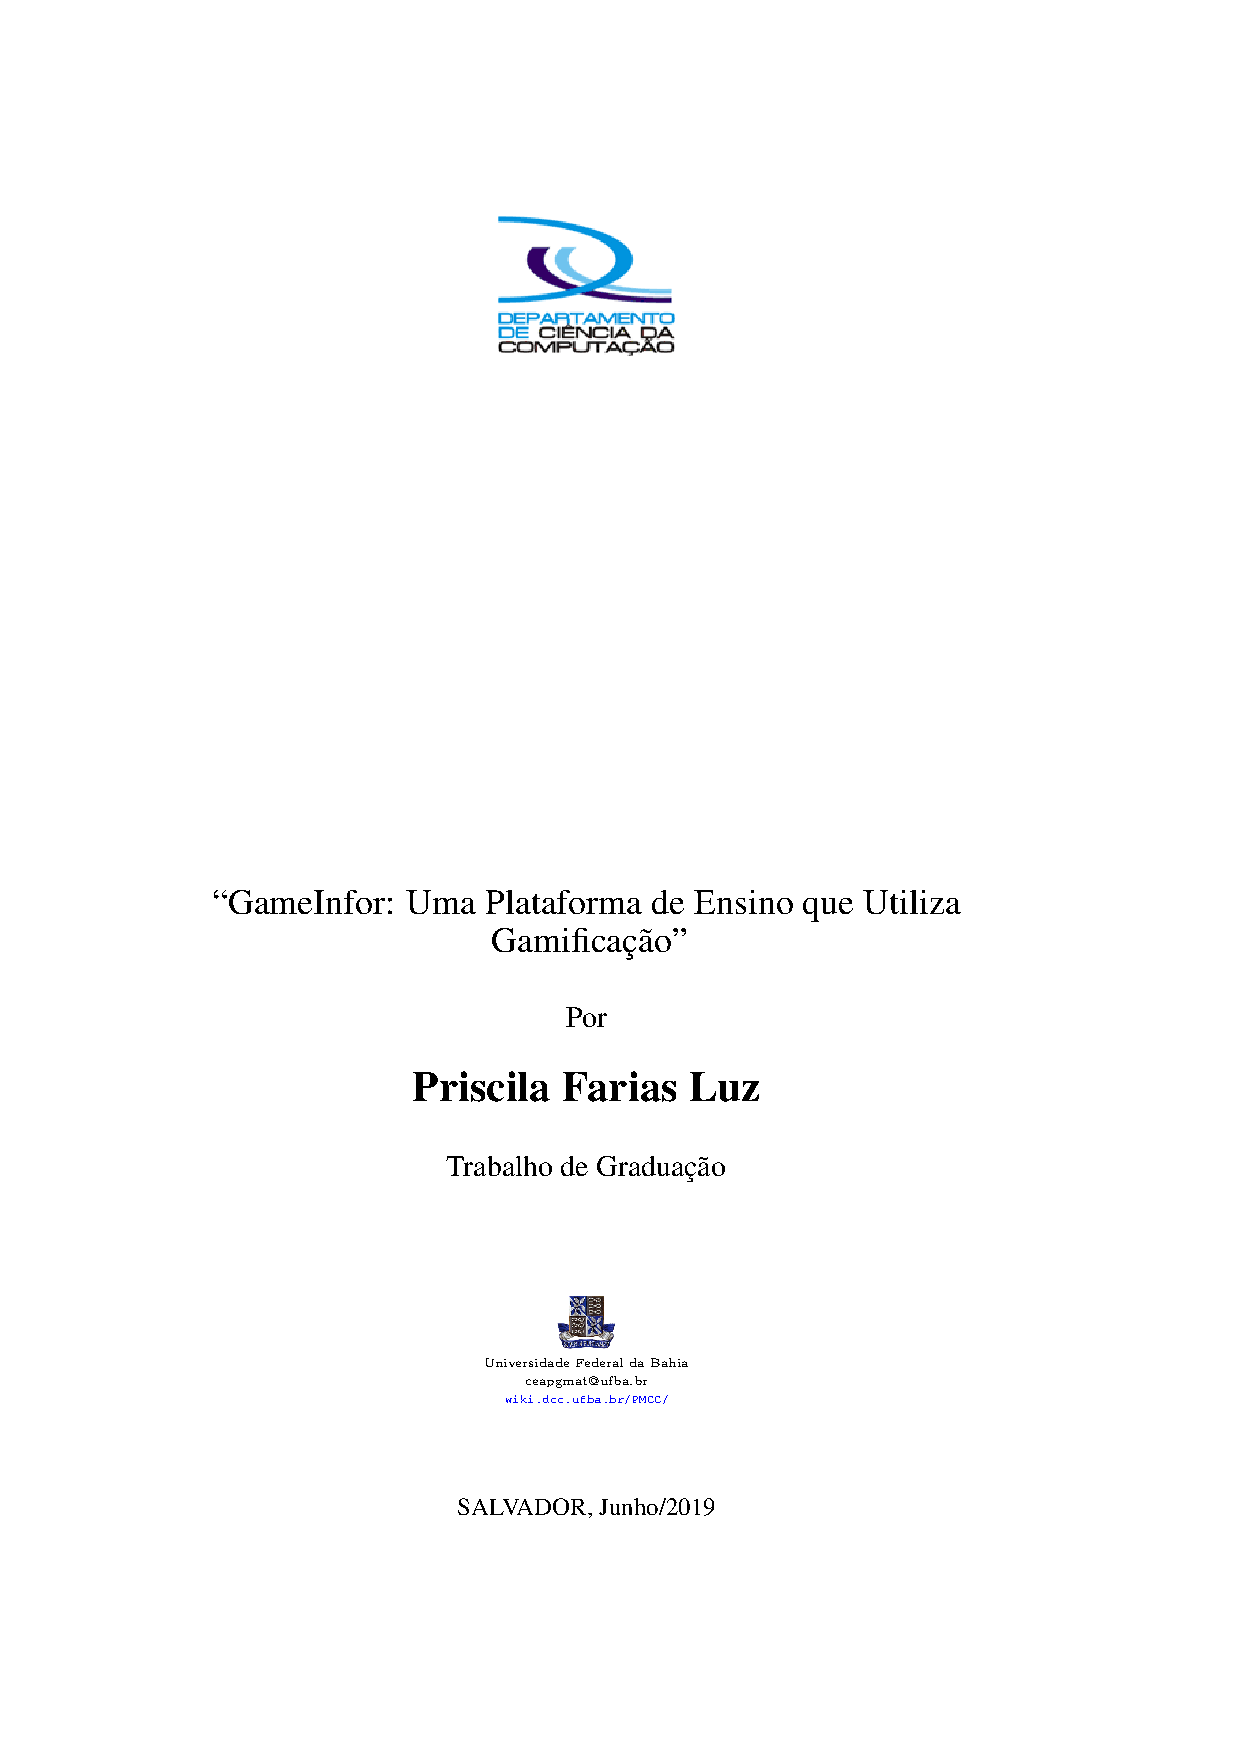
\includegraphics[width=16cm]{chapters/proposed_solution/img/captures/main.PNG}
  \caption[SPLICE main screen]{SPLICE main screen}
  \label{fg:splice-main-screen}
\end{center}
\end{figure}
The main interface can be seen in \figref{fg:splice-main-screen}, this present the main structure of the \ac{SPLICE} user interface. The main fields of are:
\begin{itemize}
\item  1. \textbf{ Tool bar.} In this part of the tool are displayed the tools and screens accessible to the user, depending on his credentials. An unlogged user, will access a limited set of options, sticking to \textit{NFR7 - Security} , providing protection to privileged information.

\item  2. \textbf{ Search bar.} It implements the functional requirement \textit{FR9 - Artifacts search}  This is the part of the tool in which the user can insert search terms and all the artifacts such as Issue Reports that contains the term will be presented to the user.
\item  3.\textbf{ Breadcrumbs.}
In this part of the tool are presented some information about the environment and some utilities. Through the toolbar, users can view information about the logged user and the actual path.
\item  4.\textbf{ Primary content.} This is the core view for content. In the \ac{SPLICE}, as default, the first screen is a collaborative document (known as \textit{Wiki page}), as shown in \figref{fg:splice-main-screen}. \textit{Wikis} implements the functional requirement \textit{FR8 - Collaborative documentation}.
\end{itemize}


\begin{figure}[htp]
\begin{center}
  \includegraphics[width=14cm]{chapters/proposed_solution/img/captures/asserts.PNG}
  \caption[SPLICE metamodel assets]{SPLICE metamodel assets}
  \label{fg:splice-metamodel-assets}
\end{center}
\end{figure}

\subsubsection{Metamodel}


The \figref{fg:splice-metamodel-assets} shows the Metamodel assets screen, and is where the requirement\textit{ FR3 - Metamodel Implementation} is represented. This screen is completely auto-generated based on the models descriptions. For every model, a complete "\acf{CRUD}" system is created, but idiosyncrasies can be easily customized. The \ac{SPLICE} also provide advanced features such as filtering and classification. In \figref{fg:splice-feature-filtering} is shown the list of indexed features, and in the side-panel is possible to filter features by \textit{Type} and \textit{Variability}.

\begin{figure}[htp]
\begin{center}
  \includegraphics[width=14cm]{chapters/proposed_solution/img/captures/View-features.PNG}
  \caption[SPLICE feature filtering]{SPLICE features filtering }
  \label{fg:splice-feature-filtering}
\end{center}
\end{figure}

\subsubsection{Issue Tracking}

Following the functional requirement \textit{FR4 - Issue Tracking}, in \figref{fg:splice-issue-tracking} it is shown a screen of ticket creation.  A ticket is defined as a software artifact that describes some defect, enhancement, change request, or an issue in general, that is submitted to an issue tracker. The \ac{SPLICE} thanks to the \textit{trac} core, have a full-featured Issue Tracking. One important addition to improve traceability in \ac{SPLICE} is the ability to close and to reference \textit{Tickets} during a commit to the \ac{VCS} by mentioning it on the commit description. Making possible to trace back the set of changes related to an Issue.

\begin{figure}[htp]
\begin{center}
  \includegraphics[width=14cm]{chapters/proposed_solution/img/captures/Ticket.PNG}
  \caption[SPLICE Issue tracking]{SPLICE Issue tracking }
  \label{fg:splice-issue-tracking}
\end{center}
\end{figure}

\subsubsection{Traceability}
\begin{figure}[htp]
\begin{center}
 \includegraphics[width=16cm]{chapters/proposed_solution/img/captures/Feature_Deatail.png}
  \caption[SPLICE Feature Traceability]{SPLICE Feature Traceability}
  \label{fg:splice-traceability}
\end{center}
\end{figure}
Implementing the requirement \textit{FR1 - Traceability}, \figref{fg:splice-traceability} depicts a \textit{Feature} report. The \ac{SPLICE} provides total traceability for all assets in the metamodel, and is able to report direct and indirect relations between them. In reports, asserts have hyperlinks, enabling the navigation between them.

\subsubsection{Product Selection}
\begin{figure}[htp]
\begin{center}
  \includegraphics[width=16cm]{chapters/proposed_solution/img/captures/Product.PNG}
  \caption[SPLICE Product edit]{SPLICE Product edit }
  \label{fg:splice-product}
\end{center}
\end{figure}

The \ac{SPLICE} have a set of custom widgets to represent specific \ac{SPL} models. One example is presented in \figref{fg:splice-product}. It depicts a modification of a \textit{Product} item. A product according to the metamodel presented in \secref{sc:metamodel} is composed of a \textit{Name}, \textit{Description} and a set of \textit{Features}. Those \textit{Features} have a number of rules and restriction, such as: “Ownership”; “Dependency”; and “Exclusion”. The custom checkbox tree control is able to handle those cases, representing the features as a tree, and automatically checking or unchecking related Features.


\subsubsection{Change history and Timeline}
\begin{figure}[htp]
\begin{center}
  \includegraphics[width=16cm]{chapters/proposed_solution/img/captures/changestory.PNG}
  \caption[SPLICE Change history]{SPLICE change history}
  \label{fg:splice-change-history}
\end{center}
\end{figure}

\begin{figure}[htp]
\begin{center}
  \includegraphics[width=16cm]{chapters/proposed_solution/img/captures/splice-timeline.PNG}
  \caption[SPLICE Timeline]{SPLICE Timeline }
  \label{fg:splice-timeline}
\end{center}
\end{figure}


The \ac{SPLICE} have a rich set of features to visualize how the project is going, where the changes are happening, and who did it. Following the functional requirement \textit{FR2 - Reporting of lifecycle artifacts}, for every Issue or Asset, a complete Change history is recorded. As \figref{fg:splice-change-history} show, the user, date/time and the performed action is automatically registered.
\figref{fg:splice-timeline} shows a timeline that the \ac{SPLICE} created containing all tickets transactions, \ac{VCS} Change-sets and documentation changes. 


\subsubsection{Control Panel}
\begin{figure}[htp]
\begin{center}
  \includegraphics[width=16cm]{chapters/proposed_solution/img/captures/config.PNG}
  \caption[SPLICE Control Panel]{SPLICE Control Panel }
  \label{fg:splice-controlpanel}
\end{center}
\end{figure}

\figref{fg:splice-controlpanel} shows the \ac{SPLICE} control panel. As the requirement \textit{FR7 - Unified User management} demands, it aggregates the configuration of all external tools in a unified interface. \figref{fg:splice-controlpanel} depicts specifically the user-account management. With the same credentials, the user is able to access all \ac{SPLICE} features, including external tools as \acf{VCS}. 

\subsubsection{Agile Planning}
\begin{figure}[htp]
\begin{center}
  \includegraphics[width=16cm]{chapters/proposed_solution/img/captures/Feature_rank.PNG}
  \caption[SPLICE agile feature rank]{SPLICE agile feature rank }
  \label{fg:splice-feature-rank}
\end{center}
\end{figure}

The \ac{SPLICE} supports a set of Agile practices as required by the \textit{FR5 - Agile Planning} requirement and is depicted in \figref{fg:splice-feature-rank}. It shows an effort estimation, where team  members  use effort and degree of difficulty to estimate their own work. The \textit{Features} can be dragged by the mouse, and their position is updated in accordance. 



\subsubsection{\acf{VCS} view}
\begin{figure}[htp]
\begin{center}
  \includegraphics[width=16cm]{chapters/proposed_solution/img/captures/splice-gitandsvn.PNG}
  \caption[SPLICE VCS view]{SPLICE Repository view}
  \label{fg:splice-vcsview}
\end{center}
\end{figure}

Following the {FR6 - Configuration management} functional requirement specification, in \figref{fg:splice-vcsview} can be seen the \ac{SPLICE} \ac{VCS} repository browser. In this figure, two different kinds of \ac{VCS} are running simultaneously,  \textit{SVN} and \textit{Git}.
In this tool, is possible to  view the log of any file or directory or a list of all the files changed, added or deleted in any given revision. Is possible to see the differences (diff) between two versions of a file so as to see exactly what was changed in a particular revision.


\subsubsection{Automatic reports generation}

\begin{figure}[htp]
\begin{center}
  \includegraphics[width=8cm]{chapters/proposed_solution/img/captures/zipped.PNG}
  \caption[SPLICE compressed reports]{SPLICE compressed reports }
  \label{fg:splice-zipped}
\end{center}
\end{figure}


\begin{figure}[htp]
\begin{center}
  \includegraphics[width=16cm]{chapters/proposed_solution/img/captures/report.PNG}
  \caption[SPLICE PDF report]{SPLICE PDF report }
  \label{fg:splice-reports}
\end{center}
\end{figure}




Based on the functional requirement \textit{FR2 - Reporting of lifecycle artifacts}, the \ac{SPLICE} have the capacity of creating reports, including \textit{PDFs}, the \textit{de facto} standard for printable document. The generated report is depicted on \figref{fg:splice-reports} and includes a cover, a summary and the set of the chosen artifact related to the product. This format is suited for presenting to the stakeholders for requirements validation. The tool is also able to collect all reports for a given Product, and create a compressed file containing the set of generated reports, as can be seen in \figref{fg:splice-zipped}. 








\section{Summary}
\label{sc:splicesummary}

In this chapter, it was presented a web-based tool for \ac{SPL} lifecycle management, including the set of functional and non-functional requirements, architecture, frameworks and technologies adopted during its construction.
Furthermore, it presented the proposal for an lightweight metamodel that represents the interaction among asserts of a \ac{SPL} during its lifecycle.
Next chapter presents a case study performed during the development of a private project.




